%!TEX root = ../template.tex

\chapter{Prototype Implementation}
\label{cha:elaboration_plan}

This chapter presents a detailed explanation of the implementation of the prototype - A Trusted and Privacy-Enhanced In-Memory Data Store, and all the implementation details that helped the system to achieve a secure state according to the adversary model.

Section \ref{sec:architecture_implementation_options} explains the system model presented on figure \ref{fig:system_model_overview} from a developer view, and presents all used technologies, programming languages and implementation details used to achieve the desired system.

Section \ref{sec:additional_details} presents some general additional security and implementation features also worth mentioning and in section \ref{sec:tradeoffs_implementation_options} it is explained some tradeoffs decided in the implementation of the prototype, and why where they made. 

To finalise, there is a general summary if the chapter in section \ref{sec:chapter4_summary} that gathers all important implementation features from all components.

The implemented prototype source code is available publicly on GitHub, secure datastore \cite{thesis-repository:container}, the proxy \cite{thesis-repository:proxy} and the client/tester \cite{thesis-repository:client} and a list of all technologies and corresponding versions are present in annex \ref{ann:technologies_and_versions}.

\section{Architecture and Implementation Options}
\label{sec:architecture_implementation_options}

To achieve the goal of deploying the system in a cloud, we had to find a provider that has and provides host machines with the pretended \gls{TEE} technology - Intel's Software Guard Extensions (\gls{SGX}v1) version 2.5.0. Although not globally available, some cloud providers are starting to make them available and for this thesis, the cloud provider used is OVH Cloud \cite{ovhcloud:1}. 

For this thesis, OVH provided an IaaS stack machine running Ubuntu Server version 18.04 with kernel 4.15.0-101-generic, which means that we have control over all host's stack but the hardware, from the operating system, networks, runtime and applications. The used machine specific configurations are listed on listing \ref{lst:ovh_machine_specs}.

\lstset{numbers=none, caption=Machine Specifications, label=lst:machine_specs}
\label{lst:ovh_machine_specs}
\begin{lstlisting}
Dedicated Server Node
Processor: Intel 2x Xeon Silver 4214 - 24c/48t - 2.2GHz/3.2Ghz
Memory: 192 GB
Hard Drive: NVMe, SATA available
Public Network: Beginning at 1 Gbps
Private Network: Beginning at 2 Gbps
CloudLinux (Ubuntu 18.04 LTS Server 64 bits)
\end{lstlisting}

This particular Intel processor offers \gls{SGX} with an 128\gls{MB} of enclave page cache (\gls{EPC}) with about 94\gls{MB} being available for application use like explained in section \ref{ssec:circumvention_of_sgx_limitations} and all \gls{SGX} linux drivers and \glspl{SDK} were installed \cite{sgx_drivers:1, sgx_sdk:1}.

All components of the application will be deployed using Docker v19.03.6 \cite{docker:1} and the Docker Compose tool v1.17.1 \cite{docker-compose:1}. To integrate and run unmodified applications with \gls{SGX}, the SCONE v4.2.1 \cite{scone:1} technology was used, and will wrap all components that need to run within a secure and isolated environment.

\subsection{Secure Redis}
\label{ssec:secure_redis}

Redis \cite{redis:1} is the key-value storage server used by this thesis. Redis instances will run in two different modes, as explained in section \ref{ssec:key-value_storage_server}. Unsecure Redis configuration will run on unprotected memory on a docker image based on the official Redis Docker repository \cite{redis:6}. For the secure configuration, SCONE framework already provides a curated image from their repository which contains a Redis server version 6.0.8 ready to run on an isolated environment, in this case Intel's SGX. The SCONE version used is the SCONE 4.2.1 to match across all the SCONE components.

Although all redis servers run behind a proxy all the necessary security features provided natively by the server are used. Only communications incoming from the proxy server are allowed and all are encrypted with strong \gls{TLS} 1.3 \footnote{TLS is a new feature released in Redis v6.0} protocols with enclave termination. The non encrypted communication port is disabled, and mutual \gls{TLS} authentication is turned on, which means that all clients are required to provide a certificate signed by the thesis CA in order to establish a connection.

Access Control is also enabled through an explicit \gls{ACL} \footnote{Redis ACL is a new feature released in Redis v6.0}. Following the principle of least privilege, users are defined via an username and a strong password and have permissions to access only the operations that they require to function.

When running in a replicated environment, master-slave or cluster, the same principles apply. Communication between replicas is also always through mutual \gls{TLS} authentication, even in cluster mode where an event bus is necessary for replica synchronisation. Replicas are read-only and since they can connect to the master instance, they use a specific user with permissions to perform just the operations that the replica needs to synchronise, and cannot alter the state of the master instance.

\subsection{Proxy Server}
\label{ssec:proxy_server}

The proxy server is the component that abstracts the Redis configurations in the backend. Proxy is a spring boot starter, version 2.3.0.RELEASE, web server application written in Kotlin v1.4.10, a language that runs on the \gls{JVM} with Java OpenJDK version 1.8.0\_222.

This component serves as a single point of entry to the system, and clients connect to it via an exposed \gls{HTTP} \gls{API} via a \gls{SSL}/\gls{TLS} encrypted channel (\gls{HTTPS}). This connection only authenticates the server, but users need to provide an authorisation header to access the server. The bearer token, on the format of a \gls{JWT} (Json Web Token) must be provided by the external authentication server as the proxy will check with it to validate the request. Not all users can access all endpoints, and the proxy decides the access control based on the role presented in the token.

Using an external configuration file, the proxy is able to communicate with multiple configurations of Redis instances. Communication with the instance is performed via Jedis v3.3.0 \cite{jedis:1}, a simple and lightweight java Redis client. When connecting to a protected Redis instance, an instance secured by \gls{SGX} processor and running inside an enclave, the proxy passes through the keys and values to the instance without any modification, meaning that values are secured inside the enclave even though they are handled in plaintext. However, all data residing on unprotected memory should be encrypted and by enabling a flag in the configuration file, the proxy will encrypt, sign and perform integrity checks on all keys and values. The homomorphic encryption is performed with the help of the Hlib v1.2r2 \cite{homolib:1}, an homomorphic encryption library implemented by the NOVA LINCS developers.

Keys for all value formats (simple, lists, etc..) are always encrypted with the Homomorphic Deterministic (HomoDet) cipher, that guarantees the same encrypted string for the same clear text value. This allows for Redis to match a given key with one present in the storage without revealing the actual value of the key.

The value from the key-value pair is encrypted in a more complex way than the keys, and their format is detailed in \ref{eq:redis_value_encrypted}, \ref{eq:redis_value_signature} and \ref{eq:final_redis_value}.

\begin{eqnarray}
EncryptedValue \  = \  [\: value \: ] \: \textsubscript{Ks} \label{eq:redis_value_encrypted} \\
CompositeValue \  = \  [\: value \: ] \: \textsubscript{Ks} \quad | \quad [\: EncryptedValue \: ] \: \textsubscript{Ksignature} \label{eq:redis_value_signature} \\
\![\: value \: ] \: \textsubscript{Ks} \quad | \quad [\: EncryptedValue \: ] \: \textsubscript{Ksignature} \quad | \quad [ \: CompositeValue \: ] \: \textsubscript{KHmac} \label{eq:final_redis_value}
\end{eqnarray}

The value is encrypted in one of two ways - refering to \ref{eq:redis_value_encrypted}:

\begin{itemize}
  \item \textbf{If the value is a string}, it is encrypted with a strong \gls{AES} cipher working on a \gls{ECB} (Electronic Code Book) mode with a \textit{PKCS5} Padding (\textit{AES/ECB/PKCS5Padding}) from SunJCE provider, with a 256 bit key.
  \item \textbf{If the value is an integer/long/double}, the value is encrypted with the Homomorphic Addition (HomoAdd) cipher from the Hlib library with a Paillier Key.
\end{itemize}

Strings are encrypted with the strongest cipher because no operation will be performed over the encrypted value, but for arithmetic values, the HomoAdd cipher is used, to allow for addition, subtraction and multiplication operations over the encrypted value.

Regardless of the encryption cipher, the encrypted value is signed with a standard SHA512 with \gls{RSA} signature algorithm from the \textit{SunRsaSign} provider - \ref{eq:redis_value_signature}. The signature is performed over the encrypted value to allow the homomorphic operations results being sign without having to decrypt the value. The signature is then appended to the encrypted value and the result is  hashed with a HMacSHA256 algorithm to provide a rapid integrity check. The result of all security operations, encryption, signature and hashing is appended into one string and set into the Redis database as a single value.

When setting a value in a list with a score, the keys and values are secured like explained above, but the scores can also pretend to sensitive data and are also encrypted. However, to provide the capabilities of fetching values between scores, a score is encrypted with the HomoOpeInt cipher from Hlib, an order preserving cipher. This cipher kepts the scores confidential but still preserves order and can be searchable on an inequality operation, for example $ x < score < y $, that fetches all values with scores between an \textit{x} and a \textit{y} number.

For demonstration purposes, when adding a value to a set, on the respective endpoint, the value is encrypted with the HomoSearch cipher from Hlib. This cipher allows searching an encrypted value for a specific substring provided by the client.

The \gls{API}, endpoints and parameters, are completely documented and available on an OpenAPI v3.0.0 \textit{yml} format.

\subsection{Client-based Benchmarks}
\label{ssec:client_based_benchmarks}

As explained before, the client is going to be emulated by a tester. Benchmarks were performed in two different ways: directly against the Redis instances, using the \textbf{redis-benchmark} \cite{redis_benchmark_cli:1} tool, and through the proxy \gls{API}.

This proxy \gls{API} tester is implemented using the Gatling v3.2.1 \cite{gatling:1} framework. Gatling is a load and performance testing tool that is configured as code. The configuration of the tool is written in Scala v2.12.3 and provides a very configurable \gls{API}. It has the ability to generate fields, that will be used to populate the database, and perform as much requests as needed or perform request during  a certain amount of time. This framework also allows to perform the necessary login request to the external authentication server in order to provided the access token to the proxy API.

For performance and load testing we can also make various simultaneous users perform actions at the same time and set up ramp up periods of higher load.

The benchmarks are doing requests to every endpoint available, and will compared against other proxy and database configurations and Gatling provides a detailed report for each one, exposing different metrics that will be presented further down this document in chapter \ref{cha:validation_experimental_Evaluation}.

Also, the same tests were configured on the Apache Jmeter v5.3\cite{jmeter:1} load testing platform to corroborate some results.

To record memory and \gls{CPU} statistics, a script written in bash was implemented that makes use of the Docker command \textit{docker-stats} to record the statistics in real time and write it to disk in a \gls{CSV} format.

\subsection{Authentication Server}
\label{ssec:implementation_authentication_server}

The external authentication server is Keycloak v10.0.2 \cite{keycloak:1}, open source identity and access management from Red Hat. This service implements the current standards for single sing-on, authentication and authorisation security.

Communication is performed over encrypted \gls{HTTPS} channels, and the client logins directly against this server to obtain the access token necessary to access the proxy.

User and roles management is done via the Keycloak user console and the platform allows for the configuration of different access token signing keys, their expiration date and supports token revocation and key rotation.

\subsection{Attestation}
\label{ssec:implementation_of_attestation}

Attestation is the mechanism responsible to provide the user with a trusted indication of the complete system state and is performed with two different methods, in two different scenarios. The hardware and \gls{SGX} attestation and an on-demand software and system stack attestation

\textbf{\gls{SGX} attestation} is performed at startup and its transparent and automatic using physical \gls{SGX} \gls{EPID}-based attestation between the application, a locally deployed attestation service (SCONE \gls{LAS}) and the remote SCONE \gls{CAS}. 

The SCONE Configuration and Attestation Service (\gls{CAS}) is a part of the system's infrastructure and it is meant to hold application secrets and injected into authenticated and attested enclaves. This service is also running inside an enclave so, any secrets stored in the server are also isolated and protected from outsiders. Each secret has a strong access policy attached and guarantees that only the right enclave, running the correct code in the correct system can access them. On application start-up, the created enclave communicates with the CAS to fetch the necessary secrets for the application to start. This is the first step of the application process and it is described in figure \ref{fig:attestation_flow}. 

\begin{figure}[htbp]
  \centering{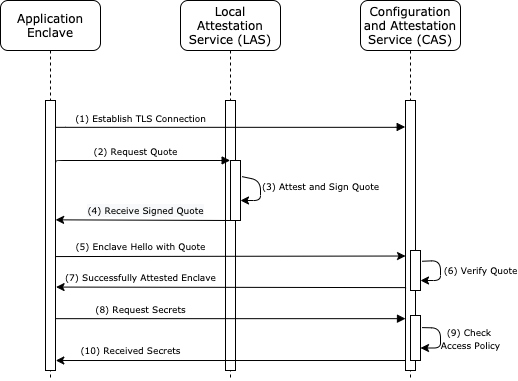
\includegraphics[width=1.0\linewidth]{SconeAttestationFlow}}%
  \caption{Attestation Flow}
  \label{fig:attestation_flow}
\end{figure}

Having established a connection with \gls{CAS} (\textbf{1}), the application now contacts the SCONE Local Attestation \footnote{Check local attestation process on annex \ref{ann:sgx_local_attestation}} Service is order to receive a signed quote from the trusted \gls{LAS} (\textbf{2, 3, 4}) that then sends to the \gls{CAS} (\textbf{5}). This quote contains information about the application enclave signed by the trusted \gls{LAS}, including and most important, the enclave hash, an hash determined by content of the pages of the enclave. \gls{CAS} can now verify the quote provided (\textbf{6} and return a success message (\textbf{7}) ff the quote is deem correct and signed by \gls{LAS}. Then, the application request the secrets from \gls{CAS} (\textbf{8}) and if the request passes all access policies (\textbf{9}), the secret is then returned (\textbf{10}) and injected into the enclave. These secrets can be injected as an environment variable or a file in a provided path, but whatever the format, they always stay inside the enclave protected memory, which means that no human or process, regardless of their roles in the system will be able to access them. on enclave destruction, the secrets are also destroyed and never written to disk or persisted anywhere. 

In case of the Redis storage server, the \gls{TLS} private keys and certificates are stored in \gls{CAS} and not in the container. This guarantees that, if it is able to provide the right certificates on a \gls{HTTPS} connection, the enclave was attested and its correct. For the Redis custom attestation service, the secrets hidden in \gls{CAS} are the quote signing keys and for the proxy server, the \gls{TLS} and the attestation signing keys as well, and the same trustability principles applies.

\textbf{The application software and stack attestation} relies on the first type attestation in order to access the keys necessary to operate, and it is performed at user request. This attestation is meant to attest binaries, config files, hardware and \gls{OS} information to the client by providing signed hashes of those resources. The client then decides if they match and pass the expected integrity checks, and if sign with a key provided by the \gls{CAS}.

This attestation service was implemented in C++14 for the Redis instances, compiled using \textit{Linux Musl g++} GNU Compiler Collection (GCC) version 10.2.0 using the Linux Chilkat C/C++ Library v9.5.0.84 statically linked to the code in order to run totally inside the enclave, and Kotlin for the proxy server. An example of the attestation response is presented in annex \ref{ann:software_stack_attestation_response_example}.

\section{Additional Details}
\label{sec:additional_details}

\subsection{Protected Memory Check}
\label{ssec:protected_memory_check}

SCONE framework says that it is running the applications inside secure enclaves and application memory is protected and there are two ways to verify it. By running an application with secrets in the SCONE configuration and attestation server (\gls{CAS}), we can be sure that the program is running inside an enclave since CAS requires a specific \gls{SGX} attestation mechanism. 

On a lower architecture level we can actually inspect the memory being used by the application. To test this, we can write a simple C program that holds a secret on an array in memory and dumping the memory of the process via the \textit{/proc} filesystem. The \textit{/proc/<pid>/map} shows the different memory regions of the process and \textit{/proc/<pid>/mem} holds the memory. By analysing this path, we can check that the secret is \textbf{not} present, as opposed to the same program running outside protected memory \cite{scone:debug}.

\subsection{Protected Heap and Stack Memory}
\label{ssec:protected_heap_and_stack_memory}

The application stack and heap memories are a core feature of any program. Stack is a memory region that stores temporary variables and data for a single computing task or function. In this memory space, variables are declared stored and initialised during runtime and are automatically erased after the code block is complete. The heap on the other hand, is a bigger region of memory, mostly allocated at startup and it stores long lived global variables, class references and other data necessary for the complete lifecycle of the program.

Running on an enclave, all of this memory must be protected and isolated from the all the other system software, hardware and even users with privileged accounts by running being placed inside the \gls{EPC}. Since we are running Intel's \gls{SGX} version 1 processors, all protected memory must be allocated at enclave startup. SCONE provides environment variables that can be set when running an application to adjust the size of the heap and stack memory regions, the SCONE\_HEAP and SCONE\_STACK variables.

Version 1 of \gls{SGX} technology means that no on-demand dynamic scaling or paging is available on the enclave allocated memory (which will be fixed by \gls{SGX}v2) and that SCONE cannot estimate how much memory the application will need. However, swapping enclave pages to main unprotected memory is still available, meaning that we can allocate more memory than the psychical \gls{EPC} limit of 128\gls{MB}, but also means that all memory must be allocated at enclave startup which can generate a higher startup time, and some \gls{OOM} (Out Of Memory) errors if the application reaches Stack or Heap allocated memory limits.

\subsection{TLS, HTTPS and Certificate Chain}
\label{ssec:tls_https_certificate_chain}

All communications in the system, both from outside or inside the system are performed over \gls{HTTPS}, \gls{TLS} v1.2 or v1.3, with custom and different certificates for each component. However, we can establish a chain of trust by signing all all certificates with a root custom certificate authority (\gls{CA}). A custom \gls{CA} was created, and signed all certificates and keys and marked as a trusted certificate authority for the entire system.

\subsection{Logging and Auditing} 
\label{sec:logging_and_auditing}

All operations in the system, being logins, proxy standard operations or even attestation requests are logged. A log line contains a timestamp, remote \gls{IP}v4 address, request information such as path, method, and response status, and the request owner, the user. However, to protect preserve privacy, username is hashed. A system administrator can access the logs in order to audit the system.

\section{Tradeoffs on the Implementation Options}
\label{sec:tradeoffs_implementation_options}

Tradeoff is the loss a system property is exchange of another. When implementing additional security properties in a system, there will always be a performance impact. It is then up to testing and use case evaluation to decide whether or not the security increase compensates the performance decrease.

When it comes to replication, there is also a decision to make referring to a consistency-performance tradeoff. Being a key-value store, Redis is always focused on performance and that is why, it follows an eventual consistency model on replication, meaning that a Redis master node will propagate changes to their slave nodes but will not wait for slave acknowledge to respond to the client.

\gls{SGX} technology also makes several tradeoff between performance and security, although it default to the latter. Protected memory size is a big issue to an \gls{SGX} enabled application, because, as explained in section \ref{ssec:circumvention_of_sgx_limitations}, the protected memory is limited, and when it is exceeded, protected memory is swapped to main memory. With additional encryption and decryption cycles as well as integrity checks, that as a penalty performance that can reach over 2000x. 

To explain this problem, we can use the OpenSSL library as an example: Dynamically linking a library to an enclave will incur a security level penalty because, not only the library cannot be trusted as it is part of the operating system and can be compromised, but also \gls{TLS} termination and decryption would be performed, outside the enclave. On the other hand, statically linking the OpenSSL libraries (option taken on this project) means that the enclave has the necessary libraries to perform \gls{TLS} termination inside the enclave. However, it will increase the size of the application, reducing the amount of memory that can be present inside the enclave and having to be being swapped into main memory.

Another implementation detail on the performance-security tradeoff topic are the homomorphic ciphers that the proxy implements on an unprotected Redis instance. Homomorphic encrypted values do leak some minor information to an attacker, although it is a good trade-off between security and performance. For example, order preserving ciphers although they do not leak specific values, they do leak the decrypted value order.

The security-performance tradeoff is not a static line, and it moves depending on the use case. For some applications, data must be extremely secure and performance can take a hit to maintain a strong privacy preserving system. This thesis implemented various security properties and all are evaluated in chapter \ref{cha:validation_experimental_Evaluation} to provide enough information for a user to decide whether or not it is a right solution to its own use case.

\section{Summary}
\label{sec:chapter4_summary}

To recap, Redis will server as a storage server and runs on an isolated environment using Intel's \gls{SGX} secure processor and also runs on normal unprotected memory. However, both solutions preserve privacy and integrity, either by \gls{SGX}'s guarantees or by proxy enabled encryption and security properties. The proxy enables some Redis out-of-the-box operations, but also some additional operations. When Redis is running in unprotected mode, the proxy enables the performance of operations over encrypted memory, sparing encryption and decryption cycles.

Both Redis and the Proxy Server are attested at start-up, by requesting application secrets hold by a third party server that implements strong access policies to make sure each secret is injected to the correct enclave. 

Users can also request attestation of the system on-demand, by requesting it to the Proxy server. The Proxy contacts all redis instance's attestation services, which are deployed alongside Redis, and returns binary, config files and system information that the user can analyse and have the guarantee that it is communicating with a correct system.

In regards to communication, all channels between all components are secure with the standard string TLS encryption with a system wide CA signature.

These security properties come with some tradeoffs but they all address a necessary privacy property, and the next chapter will evaluate them and determine if there is a bearable overhead in order to implement a secure correct and trustable system.